\apendice{Especificación de Requisitos}

\section{Introducción}
La especificación de requisitos establece el marco de trabajo para entender y documentar las necesidades del cliente y las características que debe cumplir el sistema. En esta fase, el equipo de desarrollo colabora con el \emph{product owner} mediante entrevistas y revisiones iterativas, con el fin de recopilar tanto los requisitos funcionales (las acciones que el sistema debe realizar) como los no funcionales (aspectos de calidad como seguridad, rendimiento y escalabilidad).

Históricamente, las metodologías tradicionales proponen una captura temprana y fija de requisitos, empleando estándares como IEEE 830 para garantizar que sean claros, completos y verificables. Por el contrario, las metodologías ágiles optan por la flexibilidad, recogiendo las necesidades en forma de historias de usuario dentro de un \emph{product backlog} vivo y priorizable.

Dado el carácter monodesarrollador de este TFG y la obligación de presentar una especificación detallada, se ha adoptado un enfoque híbrido que combina:

\begin{itemize}
  \item Una especificación clásica de requisitos funcionales y no funcionales, estructurada según estándares.
  \item Algunas historias de usuario representativas, derivadas de las entrevistas con el \emph{product owner}, para ilustrar la perspectiva ágil.
\end{itemize}


Una muestra de cómo podría ser una tabla de casos de uso:

\section{Objetivos generales}
Los objetivos definidos en ente proyecto son los siguientes:
\begin{enumerate}
    \item \textbf{Desarrollar un entorno virtual para la rehabilitación motriz mediante Unreal Engine:} que permita a los usuarios realizar ejercicios de rehabilitación de las extremidades superiores, a través de puzles adaptados a la tecnología VR. 

    \item \textbf{Monitorear el progreso de los usuarios durante las sesiones de rehabilitación:} Implementar un sistema que registre datos sobre el rendimiento de cada usuario, como el tiempo invertido, el número de movimientos realizados, la duración de las sesiones, y otros parámetros.

\end{enumerate}
\section{Catálogo de requisitos}
El presente Catálogo de Requisitos Funcionales recoge de manera estructurada todas las funcionalidades que el software debe ofrecer, conforme a las necesidades expuestas por el \textit{Product Owner} durante las sucesivas reuniones de definición del proyecto. Cada requisito ha sido validado y consensuado con el cliente para asegurar que el sistema cumple con sus expectativas y objetivos. A continuación se detallan las dos categorías de requisitos:

\subsection{Requisitos funcionales}
Este tipo de requerimiento (de ahora en adelante RF) detalla las funciones
que debe realizar el software para cumplir
con las expectativas del usuario. Es decir, se centra en qué debe hacer el
sistema y cómo. En esta categoría se encuentran:

\bigskip

\noindent
\textbf{RF-1 Gestión de partidas:} el sistema debe permitir al usuario gestionar sus partidas guardadas.  
\begin{itemize}
  \item \textbf{RF-1.1 Listar partidas:} el sistema mostrará todas las partidas asociadas al usuario.
  \item \textbf{RF-1.2 Cargar partida:} el sistema cargará la partida seleccionada por el usuario.
  \item \textbf{RF-1.3 Borrar partida:} el sistema eliminará de forma permanente la partida seleccionada por el usuario.
\end{itemize}

\bigskip

\noindent
\textbf{RF-2 Pantalla de créditos y agradecimientos:} el sistema debe mostrar una pantalla con los créditos de desarrollo y mensajes de agradecimiento cuando el usuario seleccione dicha opción desde el menú principal.

\bigskip

\noindent
\textbf{RF-3 Selección de nivel (puzle):} el sistema debe permitir al usuario seleccionar y preparar un nuevo puzle para jugar.  
\begin{itemize}
  \item \textbf{RF-3.1 Mostrar lista de puzles:} el sistema listará todos los puzles disponibles.
  \item \textbf{RF-3.2 Mostrar información del puzle:} al seleccionar un puzle, el sistema mostrará detalles y descripción del mismo.
  \item \textbf{RF-3.3 Iniciar puzle:} el sistema cargará el puzle seleccionado y preparará el entorno de juego.
  \item \textbf{RF-3.4 Mostrar resultados históricos:} el sistema mostrará estadísticas de sesiones anteriores asociadas al puzle seleccionado.
  \item \textbf{RF-3.5 Exportar resultados a CSV:} el sistema permitirá al usuario exportar en formato CSV los datos históricos mostrados.
\end{itemize}

\bigskip

\noindent
\textbf{RF-4 Sesión de juego:} el sistema debe gestionar la ejecución de la sesión de juego completa.  
\begin{itemize}
  \item \textbf{RF-4.1 Introducción narrativa:} al iniciar la sesión, el sistema mostrará una breve narrativa introductoria.
  \item \textbf{RF-4.2 Ejecución del puzle:} el sistema permitirá al usuario realizar la tarea o resolver el puzle.
  \item \textbf{RF-4.3 Mostrar estadísticas de la sesión:} al finalizar, el sistema calculará y mostrará la duración de la sesión y otras estadísticas básicas.
\end{itemize}

\bigskip

\noindent

\textbf{RF-5 Consulta de datos:} el terapeuta será capaz de consultar los datos contenidos en el CSV previamente exportado.

\subsection{Requisitos no funcionales}


Además de los requisitos funcionales, es fundamental definir las condiciones de calidad, rendimiento y restricciones bajo las cuales el sistema debe operar. A continuación se incluyen los Requisitos No Funcionales identificados:

\bigskip

\noindent
\begin{itemize}
  \item \textbf{RNF-1 Rendimiento:} Mantener al menos 72 FPS estables en Meta Quest 2 durante toda la sesión de juego.
  
  \item \textbf{RNF-2 Usabilidad:} La interfaz debe permitir completar las acciones principales (listar, cargar, borrar partidas; seleccionar e iniciar puzles; ver/exportar resultados) en un máximo de 2 gestos de controlador dentro de un alcance de brazo.
  
  \item \textbf{RNF-3 Portabilidad:} El software debe ser compatible con Meta Quest.
  
  \item \textbf{RNF-4 Fiabilidad:} La tasa de errores críticos (\textit{crash} o pérdida de datos) debe ser casi nula.
  
  \item \textbf{RNF-5 Accesibilidad VR:}  
    \begin{itemize}
      \item Soporte exclusivo de interacción sentado, sin requerir desplazamiento físico del usuario.  
      \item Todas las acciones deben realizarse mediante movimientos de extremidades superiores (controladores de mano), sin exigir movimientos de torso o piernas.  
      \item Elementos de interfaz e interactivos a una distancia máxima de 0,6 m (alcance del brazo) y a una altura entre 0,8 m y 1,5 m del suelo aproximadamente.  
    \end{itemize}
\end{itemize}
\section{Especificación de requisitos}
A continuación se presenta la especificación detallada de requisitos de la aplicación \emph{VR} desarrollada en Unreal Engine 5.5 para Meta Quest 2, basada en el Catálogo de Requisitos. En esta sección se describen en profundidad tanto los requisitos funcionales como los no funcionales, incluyendo sus precondiciones, criterios de aceptación y prioridades, con el fin de asegurar que el sistema satisfaga las necesidades de usuarios con movilidad reducida y de los terapeutas encargados de su seguimiento.

\subsection{Diagrama de casos de uso}
Tomando como base las historias de usuario definidas junto al \textit{Product Owner}, se ha construido el diagrama general de casos de uso de la aplicación. A continuación se presenta dicho diagrama, seguido de las tablas detalladas de cada caso de uso.
\begin{figure}[h]
	\caption[Diagrama: casos de uso]{Diagrama general de casos de uso de la aplicación.}
	\centering
	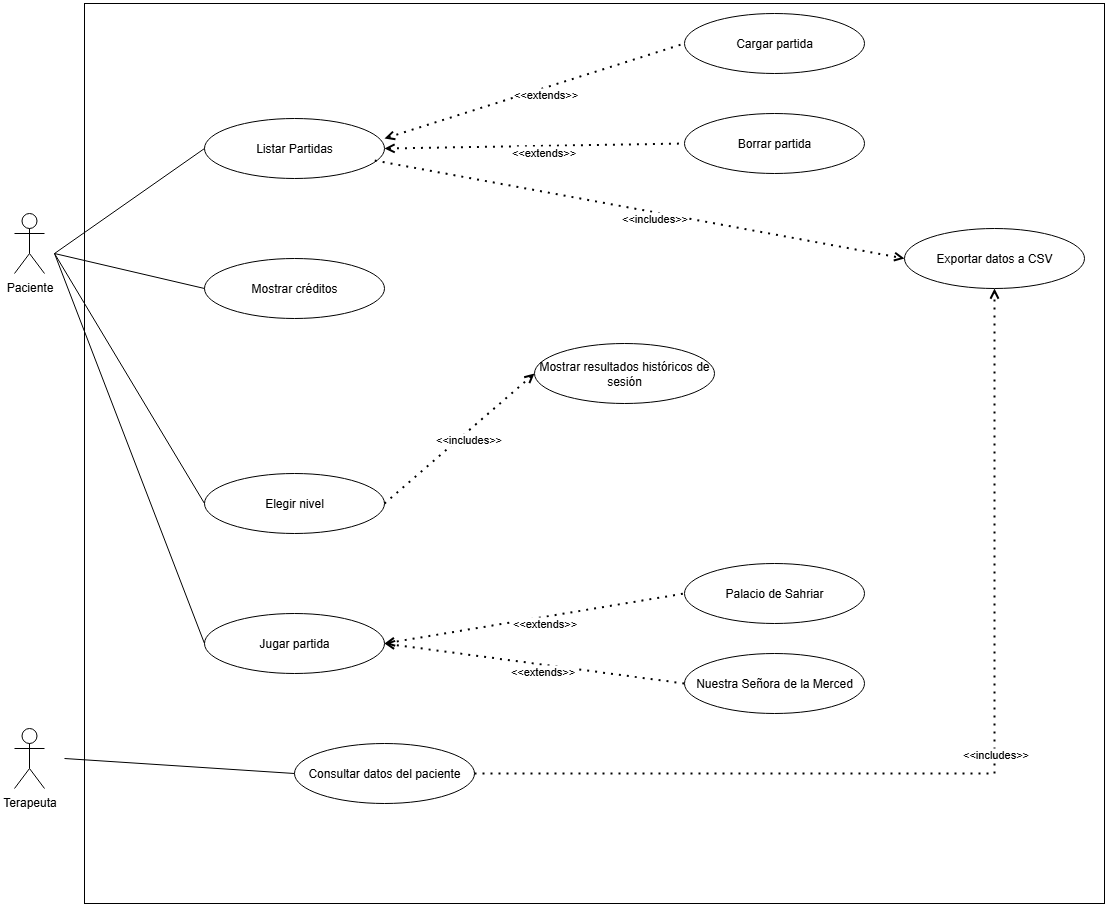
\includegraphics[width=\textwidth, keepaspectratio]{../img/anexos/diagramacasodeuso.png}
	\label{b:diagrama-cu}
\end{figure}

\begin{table}[p]
	\centering
	\begin{tabularx}{\linewidth}{ p{0.21\columnwidth} p{0.71\columnwidth} }
		\toprule
		\textbf{CU-1} & \textbf{Listar partidas}\\
		\toprule
		\textbf{Versión}              & 1.0    \\
		\textbf{Autor}                & Rodrigo Grande \\
		\textbf{Requisitos asociados} & RF-1 (RF-1.1) \\
		\textbf{Descripción}          & Permite al usuario visualizar la lista de partidas existentes asociadas a su cuenta.\\
		\textbf{Precondición}         & El usuario debe haber iniciado sesión y tener al menos una partida guardada. \\
		\textbf{Acciones}             &
		\begin{enumerate}
			\def\labelenumi{\arabic{enumi}.}
			\tightlist
			\item El usuario selecciona <<Listar partidas>>.
			\item El sistema recupera y muestra todas las partidas disponibles para el usuario.
		\end{enumerate}\\
		\textbf{Postcondición}        & Se presenta al usuario la lista actualizada de partidas. \\
		\textbf{Excepciones}          & Si no existen partidas, el sistema muestra un mensaje “No hay partidas disponibles”. \\
		\textbf{Importancia}          & Alta \\
		\bottomrule
	\end{tabularx}
	\caption{CU-1 Listar partidas.}
	\label{cu:listar-partidas}
\end{table}

\begin{table}[p]
	\centering
	\begin{tabularx}{\linewidth}{ p{0.21\columnwidth} p{0.71\columnwidth} }
		\toprule
		\textbf{CU-2} & \textbf{Cargar partida guardada}\\
		\toprule
		\textbf{Versión}              & 1.0    \\
		\textbf{Autor}                & Rodrigo Grande \\
		\textbf{Requisitos asociados} & RF-1 (RF-1.2) \\
		\textbf{Descripción}          & Permite al usuario cargar una de sus partidas previamente guardadas.\\
		\textbf{Precondición}         & El usuario debe haber iniciado sesión y existir la partida seleccionada. \\
		\textbf{Acciones}             &
		\begin{enumerate}
			\def\labelenumi{\arabic{enumi}.}
			\tightlist
			\item El usuario elige <<Lista de partidas>>.
			\item El sistema muestra la lista de partidas disponibles.
			\item El usuario selecciona la partida deseada.
			\item El sistema carga los datos de la partida seleccionada.
		\end{enumerate}\\
		\textbf{Postcondición}        & La partida guardada se carga y el usuario puede continuar jugando. \\
		\textbf{Excepciones}          & Si la partida está corrupta o no existe, se muestra un mensaje de error y se mantiene la sesión anterior. \\
		\textbf{Importancia}          & Alta \\
		\bottomrule
	\end{tabularx}
	\caption{CU-2 Cargar partida guardada.}
	\label{cu:cargar-partida}
\end{table}

\begin{table}[p]
	\centering
	\begin{tabularx}{\linewidth}{ p{0.21\columnwidth} p{0.71\columnwidth} }
		\toprule
		\textbf{CU-3} & \textbf{Borrar partida}\\
		\toprule
		\textbf{Versión}              & 1.0    \\
		\textbf{Autor}                & Rodrigo Grande \\
		\textbf{Requisitos asociados} & RF-1 (RF-1.3) \\
		\textbf{Descripción}          & Permite al usuario eliminar una partida de su cuenta de forma permanente.\\
		\textbf{Precondición}         & El usuario debe haber iniciado sesión y existir la partida seleccionada. \\
		\textbf{Acciones}             &
		\begin{enumerate}
			\def\labelenumi{\arabic{enumi}.}
			\tightlist
			\item El usuario selecciona <<Borrar partida>>.
			\item El sistema elimina la partida y actualiza la lista.
		\end{enumerate}\\
		\textbf{Postcondición}        & La partida seleccionada queda eliminada de la cuenta del usuario. \\
		\textbf{Excepciones}          & Si la eliminación falla, se informa al usuario y no se modifica la lista. \\
		\textbf{Importancia}          & Alta \\
		\bottomrule
	\end{tabularx}
	\caption{CU-3 Borrar partida.}
	\label{cu:borrar-partida}
\end{table}

\begin{table}[p]
	\centering
	\begin{tabularx}{\linewidth}{ p{0.21\columnwidth} p{0.71\columnwidth} }
		\toprule
		\textbf{CU-4} & \textbf{Mostrar pantalla de créditos y agradecimientos}\\
		\toprule
		\textbf{Versión}              & 1.0    \\
		\textbf{Autor}                & Rodrigo Grande \\
		\textbf{Requisitos asociados} & RF-2 \\
		\textbf{Descripción}          & Muestra una pantalla con los créditos del desarrollo y mensajes de agradecimiento.\\
		\textbf{Precondición}         & El usuario accede a la sección de créditos desde el menú principal. \\
		\textbf{Acciones}             &
		\begin{enumerate}
			\def\labelenumi{\arabic{enumi}.}
			\tightlist
			\item El usuario selecciona <<Créditos>> en el menú.
			\item El sistema presenta la pantalla con la información de los desarrolladores y colaboradores.
		\end{enumerate}\\
		\textbf{Postcondición}        & El usuario visualiza la pantalla de créditos. \\
		\textbf{Excepciones}          & Ninguna esperada; si falla la carga, se muestra un mensaje genérico. \\
		\textbf{Importancia}          & Media \\
		\bottomrule
	\end{tabularx}
	\caption{CU-4 Mostrar pantalla de créditos y agradecimientos.}
	\label{cu:creditos}
\end{table}

\begin{table}[p]
	\centering
	\begin{tabularx}{\linewidth}{ p{0.21\columnwidth} p{0.71\columnwidth} }
		\toprule
		\textbf{CU-5} & \textbf{Elegir nivel}\\
		\toprule
		\textbf{Versión}              & 1.0    \\
		\textbf{Autor}                & Rodrigo Grande \\
		\textbf{Requisitos asociados} & RF-3 (RF-3.1,RF-3.2,RF-3.3) \\
		\textbf{Descripción}          & Permite al usuario seleccionar un puzle para iniciar una nueva partida.\\
		\textbf{Precondición}         & El usuario debe haber iniciado sesión. \\
		\textbf{Acciones}             &
		\begin{enumerate}
			\def\labelenumi{\arabic{enumi}.}
			\tightlist
			\item El usuario elige <<Nueva partida>>.
			\item El sistema muestra la lista de puzles disponibles.
			\item El usuario selecciona el puzle deseado.
			\item El sistema muestra información detallada del puzle.
			\item El usuario pulsa <<Botón con el nombre de puzle>>.
			\item El sistema carga el puzle seleccionado.
		\end{enumerate}\\
		\textbf{Postcondición}        & El puzle está listo para jugarse. \\
		\textbf{Excepciones}          & Fallo de carga de nivel, se informa al usuario con un mensaje. \\
		\textbf{Importancia}          & Alta \\
		\bottomrule
	\end{tabularx}
	\caption{CU-5 Elegir juego (nivel).}
	\label{cu:elegir-juego}
\end{table}

\begin{table}[p]
	\centering
	\begin{tabularx}{\linewidth}{ p{0.21\columnwidth} p{0.71\columnwidth} }
		\toprule
		\textbf{CU-6} & \textbf{Mostrar resultados históricos de sesión}\\
		\toprule
		\textbf{Versión}              & 1.0    \\
		\textbf{Autor}                & Rodrigo Grande \\
		\textbf{Requisitos asociados} & RF-3 (RF-3.4) \\
		\textbf{Descripción}          & Extiende CU-5 para mostrar estadísticas de sesiones anteriores del puzle seleccionado.\\
		\textbf{Precondición}         & Se ha seleccionado un puzle (CU-5). \\
		\textbf{Acciones}             &
		\begin{enumerate}
			\def\labelenumi{\arabic{enumi}.}
			\tightlist
			\item El usuario elige <<Ver resultados históricos>>.
			\item El sistema recupera los datos de sesiones previas de ese puzle.
			\item Se muestran las estadísticas (duración, puntuación) en pantalla.
		\end{enumerate}\\
		\textbf{Postcondición}        & Se visualizan los datos históricos. \\
		\textbf{Excepciones}          & Si no existen datos, se muestra “No hay resultados anteriores”. \\
		\textbf{Importancia}          & Media \\
		\bottomrule
	\end{tabularx}
	\caption{CU-6 Mostrar resultados históricos de sesión asociados al puzle seleccionado.}
	\label{cu:resultados-historicos}
\end{table}

\begin{table}[p]
	\centering
	\begin{tabularx}{\linewidth}{ p{0.21\columnwidth} p{0.71\columnwidth} }
		\toprule
		\textbf{CU-7} & \textbf{Exportar a CSV}\\
		\toprule
		\textbf{Versión}              & 1.0    \\
		\textbf{Autor}                & Rodrigo Grande \\
		\textbf{Requisitos asociados} & RF-3 (RF-3.5) \\
		\textbf{Descripción}          & Extiende CU-6 para exportar los resultados históricos a un archivo CSV.\\
		\textbf{Precondición}         & Se están mostrando resultados históricos (CU-6). \\
		\textbf{Acciones}             &
		\begin{enumerate}
			\def\labelenumi{\arabic{enumi}.}
			\tightlist
			\item El usuario selecciona <<Exportar a CSV>>.
			\item El sistema genera un fichero CSV con los datos mostrados.
			\item Se inicia la descarga del CSV al dispositivo del usuario.
		\end{enumerate}\\
		\textbf{Postcondición}        & El fichero CSV con resultados históricos está descargado. \\
		\textbf{Excepciones}          & Si hay un error en la generación, se informa al usuario. \\
		\textbf{Importancia}          & Media \\
		\bottomrule
	\end{tabularx}
	\caption{CU-7 Exportar a CSV.}
	\label{cu:exportar-csv}
\end{table}

\begin{table}[p]
	\centering
	\begin{tabularx}{\linewidth}{ p{0.21\columnwidth} p{0.71\columnwidth} }
		\toprule
		\textbf{CU-8} & \textbf{Jugar partida}\\
		\toprule
		\textbf{Versión}              & 1.0    \\
		\textbf{Autor}                & Rodrigo Grande \\
		\textbf{Requisitos asociados} & RF-4 (RF-4.1,RF-4.2,RF-4.3) \\
		\textbf{Descripción}          & Actividad principal del videojuego: incluye una introducción narrativa y la ejecución del puzle, finalizando con la presentación resumida de estadísticas de la sesión.\\
		\textbf{Precondición}         & El puzle debe estar cargado y listo para jugarse (CU-5). \\
		\textbf{Acciones}             &
		\begin{enumerate}
			\def\labelenumi{\arabic{enumi}.}
			\tightlist
			\item El sistema muestra la narrativa introductoria.
			\item El usuario realiza la tarea o resuelve el puzle.
			\item Al finalizar, el sistema calcula la duración de la sesión.
			\item Se muestran las estadísticas básicas de la sesión.
		\end{enumerate}\\
		\textbf{Postcondición}        & La sesión queda registrada con su duración y resultados. \\
		\textbf{Excepciones}          & Si hay fallo al guardar estadísticas, se notifica al usuario y se vuelve a intentar. \\
		\textbf{Importancia}          & Alta \\
		\bottomrule
	\end{tabularx}
	\caption{CU-8 Realizar sesión de juego.}
	\label{cu:jugar-partida}
\end{table}

\begin{table}[p]
	\centering
	\begin{tabularx}{\linewidth}{ p{0.21\columnwidth} p{0.71\columnwidth} }
		\toprule
		\textbf{CU-9} & \textbf{Jugar partida: Palacio de Shahriar}\\
		\toprule
		\textbf{Versión}              & 1.0    \\
		\textbf{Autor}                & Rodrigo Grande \\
		\textbf{Requisitos asociados} & RF-4 (RF-4.1,RF-4.2,RF-4.3)) \\
		\textbf{Descripción}          & Especialización de CU-8 para el escenario del Palacio de Shahriar, con narrativa y desafíos temáticos.\\
		\textbf{Precondición}         & El usuario ha seleccionado el puzle “Palacio de Shahriar” (CU-5). \\
		\textbf{Acciones}             &
		\begin{enumerate}
			\def\labelenumi{\arabic{enumi}.}
			\tightlist
			\item El sistema presenta la historia del Palacio de Shahriar.
			\item El usuario resuelve el enigma específico de este escenario.
			\item Se calculan y muestran las estadísticas de la sesión.
		\end{enumerate}\\
		\textbf{Postcondición}        & La sesión temática queda registrada con sus estadísticas. \\
		\textbf{Excepciones}          & Si falla la carga del escenario, se informa al usuario y se vuelve al menú de selección. \\
		\textbf{Importancia}          & Alta \\
		\bottomrule
	\end{tabularx}
	\caption{CU-9 Jugar partida: Palacio de Shahriar }
	\label{cu:jugar-partida-palacio-shahriar}
    \end{table}
    \begin{table}[p]
	\centering
	\begin{tabularx}{\linewidth}{ p{0.21\columnwidth} p{0.71\columnwidth} }
		\toprule
		\textbf{CU-10} & \textbf{Consulta de datos}\\
		\toprule
		\textbf{Versión}              & 1.0    \\
		\textbf{Autor}                & Rodrigo Grande \\
		\textbf{Requisitos asociados} & RF-5 \\
		\textbf{Descripción}          & El terapeuta sera capaz de consultar los datos exportados por el usuario.\\
		\textbf{Precondición}         & El usuario ha exportado los datos a CSV y este es facilitado al terapeuta. \\
		\textbf{Acciones}             &
		\begin{enumerate}
			\def\labelenumi{\arabic{enumi}.}
			\tightlist
			\item El terapeuta consulta el CSV.
		\end{enumerate}\\
		\textbf{Postcondición}        & El usuario recibe un \textit{feedback} por parte del terapeuta. \\
		\textbf{Excepciones}          & El CSV no ha sido exportado correctamente. \\
		\textbf{Importancia}          & Alta \\
		\bottomrule
	\end{tabularx}
	\caption{CU-10 Consulta de datos.}
	\label{cu:consulta-de-datos}
\end{table}
